%!TEX root=../document.tex
\section{Allgemein - Stored Routines MySQL}
MySQL 5.1 kennt auch gespeicherte Routinen (Prozeduren und Funktionen). Eine gespeicherte Prozedur ist eine Menge von SQL-Anweisungen, die auf dem Server gespeichert werden kann. So mussen Clients nicht immer wieder die jeweiligen Einzelanweisungen ausfuhren, sondern konnen stattdessen die gespeicherte Prozedur aufrufen.

Stored Routines werden folgendermasen eingesetzt:
\begin{itemize}
	\item Wenn mehrere Clientanwendungen in verschiedenen Sprachen geschrieben sind oder auf verschiedenen Plattformen laufen, aber dieselben Datenbankoperationen ausfuhren mussen.
	\item Wenn Sicherheit sehr wichtig ist. Banken verwenden zum Beispiel fur alle haufigen Operationen gespeicherte Prozeduren und Funktionen. Das gewahrleistet eine konsistente und sichere Umgebung sowie eine korrekte Protokollierung jeder einzelnen Operation. In einer solchen Umgebung haben Anwendungen und Benutzer keinen Direktzugriff auf die Datenbanktabellen, sondern konnen nur bestimmte gespeicherte Routinen ausfuhren.
\end{itemize}
Gespeicherte Routinen bieten eine bessere Leistung, da weniger Informationen zwischen Server und Client ubermittelt werden mussen. Der Nachteil ist der, dass die Belastung des Datenbankservers steigt, weil mehr Arbeit auf der Serverseite und weniger Arbeit auf der Seite des Clients (der Anwendungen) erledigt werden muss. Dies mussen Sie berucksichtigen, wenn viele Clientcomputer (wie beispielsweise Webserver) von nur einem oder sehr wenigen Datenbankservern bedient werden.
\subsection{Stored Procedures}
Stored Proceduren in MySQL unterscheiden sich von Stored Functions.
Prozeduren können nur mittels \textit{call procname} und nicht innerhalb einer \textit{select} Anweisung aufgerufen werden.

Prinzipiell können Parameter bei Prozeduren als \textbf{IN} oder \textbf{OUT} Parameter definiert werden.

Prozeduren können nur Werte mittels Output Parameter an den Aufrufer zurückliefern.

\clearpage
\subsubsection{Syntax}
\begin{lstlisting}[style=sql1]
-- Syntax/Synopsis CREATE STORED PROCEDURE
CREATE
	[DEFINER = { user | CURRENT_USER }]
	PROCEDURE sp_name ([proc_parameter[,...]])
	[characteristic ...] routine_body

proc_parameter:
	[ IN | OUT | INOUT ] param_name type
	
type:
	Any valid MySQL data type

characteristic:
	COMMENT 'string'
	| LANGUAGE SQL
	| [NOT] DETERMINISTIC
	| { CONTAINS SQL | NO SQL | READS SQL DATA | MODIFIES SQL DATA }
	| SQL SECURITY { DEFINER | INVOKER }

routine_body:
	Valid SQL routine statement
\end{lstlisting}

\subsection{Stored Functions}
Stored Functions in MySQL unterscheiden sich von Stored Prozeduren.
Functions können mittels \textit{select} Anweisung aufgerufen werden.

Functions können grundsätzlich nur mithilfe eines \textit{RETURNS} werte an den Aufrufer zurückliefern.
Grundsätzlich ist es nicht möglich ein \textbf{set of} mit mysql functions zurückzuliefern.

Functionen können keine \textbf{FLUSH} Statements verwenden, wobei Prozeduren dies sehr wohl unterstützen.

Rekursive Funktionen werden von MySQL nicht unterstützt. Prozeduren sind standardgemäß nicht rekursiv können aber mittels Änderung von bestimmten System Variables angepasst werden.
\clearpage
\subsubsection{Syntax}
\begin{lstlisting}[style=sql1]
-- Syntax/Synopsis CREATE STORED PROCEDURE
CREATE
	[DEFINER = { user | CURRENT_USER }]
	FUNCTION sp_name ([func_parameter[,...]])
	RETURNS type
	[characteristic ...] routine_body

func_parameter:
	param_name type

type:
	Any valid MySQL data type

characteristic:
	COMMENT 'string'
	| LANGUAGE SQL
	| [NOT] DETERMINISTIC
	| { CONTAINS SQL | NO SQL | READS SQL DATA | MODIFIES SQL DATA }
	| SQL SECURITY { DEFINER | INVOKER }

routine_body:
	Valid SQL routine statement
\end{lstlisting}

\clearpage

\section{Vorbereitung}
Um alle Anforderungen der Aufgabenstellung zu erfüllen müssen zuerst gewisse Vorbereitungen getroffen werden.
Bevor die eigentlichen Prozeduren erstellt werden können muss zuerst die bestehende Datenbank von psql auf mysql migriert und umgeschrieben werden.

\subsection{Anpassen des Create - Scripts}
Prinzipiell versteht PostgreSQL sowie auch MySQL den standard SQL dialekt, jedoch gibt es sehr wohl Unterschiede, welche ein problemloses migrieren des Create - Scripts nicht erlauben.

Hierbei mussten zuerst alle psql spezifischen Befehle wie \textit{/c,} durch MySQL Befehle ersetzt werden. Ansonsten konnte das Create - Script 1:1 übernommen werden, um alle Daten sowie Tabellendefinitionen in MySQL zu importieren.

Anschließend wurde nur noch das Create Script ausgeführt und die Datenbank wurde entsprechend erstellt.

\section{Ergebnisse}
Alle Ergebnisse werden untersucht und in bezug auf Postgresql verglichen. Wobei letztendlich die execution Time sowie die Schwierigkeit der Umsetzung bewertet und analysiert wird.

\subsection{AU01 - \textit{preisTo99()} \& \textit{loescheRechnung()}}
\subsubsection{Umsetzung - \textit{preisTo99()}}
\vspace{0.3cm}
\begin{minipage}{.5\textwidth}
	\begin{lstlisting}[style=sql1, caption={preisTo99() - MySQL}]
--	Alle Preise auf .99 aufrunden
DROP PROCEDURE IF EXISTS preisTo99;
delimiter //
	CREATE PROCEDURE preisTo99() 
	BEGIN
		UPDATE speise SET preis=ceil(preis)-0.01;
	END //
delimiter ;
	\end{lstlisting}
\end{minipage}%
\begin{minipage}{.5\textwidth}
	\begin{lstlisting}[style=sql, caption={preisTo99() - PSQL}]
--	Alle Preise auf .99 aufrunden
--		ceil(preis) - 0.01
--		floor(preis) + 0.99
--		trunc
CREATE FUNCTION preisTo99() returns void as '
UPDATE speise set preis = ceil(preis) - 0.01;
' language sql;
	\end{lstlisting}
\end{minipage}

\subsubsection{Umsetzung - \textit{loescheRechnung()}}
\vspace{0.3cm}
\begin{minipage}{.5\textwidth}
	\begin{lstlisting}[style=sql1, caption={loescheRchng() - MySQL}]
DROP PROCEDURE IF EXISTS loescheRchng;
delimiter //
	CREATE PROCEDURE loescheRechnung() 
	BEGIN
		DELETE from rechnung where rnr not in (
		select rnr from bestellung
		);
	END //
delimiter ;
	\end{lstlisting}
\end{minipage}%
\begin{minipage}{.5\textwidth}
	\begin{lstlisting}[style=sql, caption={loescheRchng() - PSQL}]
--	Alle Rechnungen loeschen
--		ceil(preis) - 0.01
--		floor(preis) + 0.99
CREATE FUNCTION loescheRechnung() returns void as '
	DELETE from rechnung where rnr not in (
		select rnr from bestellung
	);
' language sql;
	\end{lstlisting}
\end{minipage}

\subsubsection{Bemerkungen}
Umsetzung konnte problemlos durchgeführt werden. Einzige Unterschiede lassen sich aus der Syntax der jeweiligen Functions ersehen. Außerdum kann eine Prozedur nur mittels call aufgerufen werden.

\subsubsection{Screenshots}
\vspace{0.2cm}
\begin{minipage}{.5\textwidth}
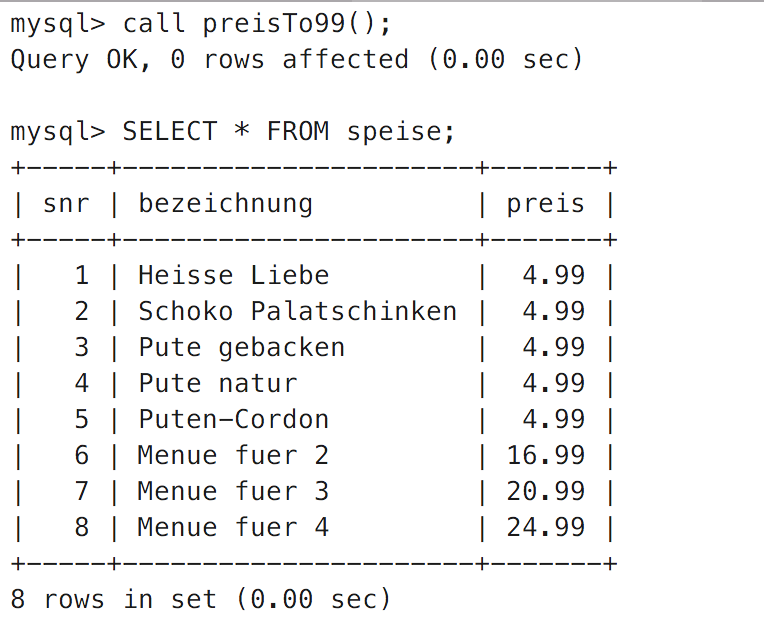
\includegraphics[width=1\linewidth]{images/s01.png}
\end{minipage}%
\begin{minipage}{.5\textwidth}
	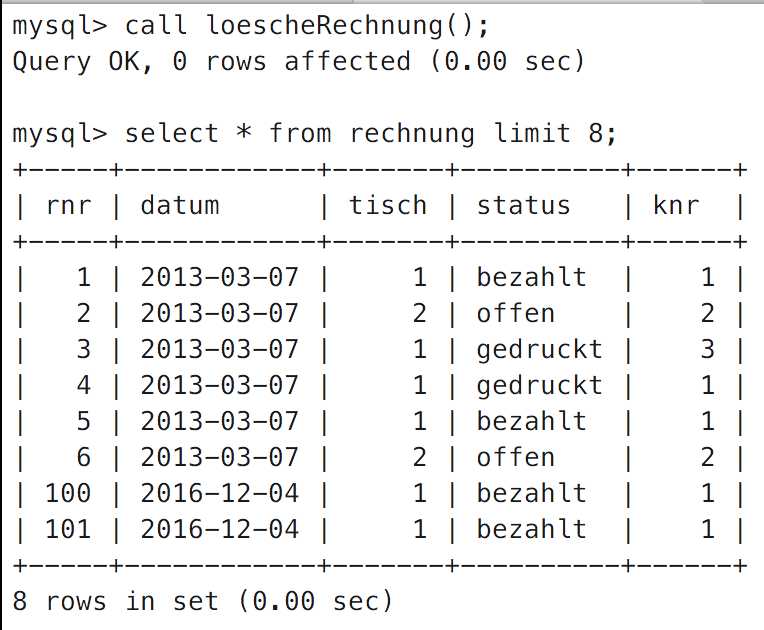
\includegraphics[width=1\linewidth]{images/s02.png}
\end{minipage}

\clearpage

\subsection{AU02 - \textit{preiserhoehung()}}
\subsubsection{Umsetzung - \textit{preiserhoehung()}}
\vspace{0.3cm}
\begin{minipage}{.5\textwidth}
	\begin{lstlisting}[style=sql1, caption={preiserhoehung() - MySQL}]
DROP PROCEDURE IF EXISTS increasePreis;
delimiter //
	CREATE PROCEDURE increasePreis(IN pr DECIMAL, IN abs INTEGER) 
	BEGIN
		DECLARE average DECIMAL DEFAULT (SELECT avg(preis) from speise);
		UPDATE speise SET preis=abs
		where preis <= average;
		UPDATE speise SET preis=preis * (100 + pr) / 100
		where preis > average;
	END //
delimiter ;
	\end{lstlisting}
\end{minipage}%
\begin{minipage}{.5\textwidth}
	\begin{lstlisting}[style=sql, caption={preiserhoehung() - PSQL}]
--	Erhoehen von ausgewaehlten Speicsen um einen spezifischen Wert	
-- Erhoehen der anderen Preise um einen Prozentwert
CREATE FUNCTION increaseAverage(DECIMAL(6,2), INTEGER) returns void as 
'
	UPDATE speise 
	set preis = preis + $2
	where preis <= $1;

	Update speise
	set preis = preis * (100 + $2) / 100
	where preis > $1;
' language sql;
	\end{lstlisting}
\end{minipage}

\subsubsection{Bemerkungen}
Ebenfalls mussen parameter bei einer prozedur mittels \textbf{IN} und \textbf{OUT} definiert werden, im Unterschied zu psql woebi es nur ''\textit{IN}'' Parameter gibt.

\subsubsection{Screenshots}
\vspace{0.2cm}
\begin{minipage}{.5\textwidth}
	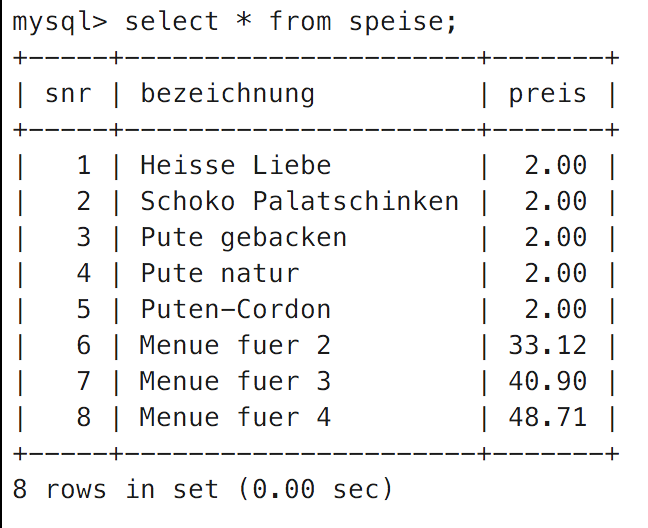
\includegraphics[width=0.9\linewidth]{images/s03.png}
\end{minipage}%
\begin{minipage}{.5\textwidth}
	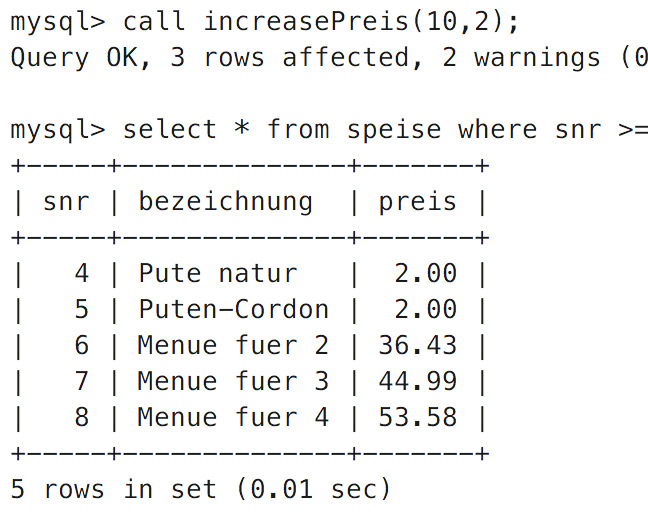
\includegraphics[width=0.9\linewidth]{images/s04.png}
\end{minipage}

\clearpage

\subsection{AU03 - Tagesumsatz je Kellner}
\subsubsection{Benoetigte Inserts}
\begin{lstlisting}[style=sql1, caption={inserts Au03 - MySQL}]
--			Inserts weil keine CURRENT-DATE Datensaetze
INSERT INTO rechnung VALUES (100, CURRENT_DATE, 1, 'bezahlt', 1);
INSERT INTO rechnung VALUES (110, CURRENT_DATE, 2, 'bezahlt', 2);
INSERT INTO rechnung VALUES (120, CURRENT_DATE, 1, 'bezahlt', 3);
INSERT INTO rechnung VALUES (130, CURRENT_DATE, 1, 'bezahlt', 1);
INSERT INTO rechnung VALUES (140, CURRENT_DATE, 1, 'bezahlt', 1);
...

INSERT INTO bestellung VALUES (1, 100, 7);
INSERT INTO bestellung VALUES (1, 110, 8);
INSERT INTO bestellung VALUES (9, 120, 1);
INSERT INTO bestellung VALUES (9, 130, 1);
INSERT INTO bestellung VALUES (9, 140, 2);
...
\end{lstlisting}
\subsubsection{Umsetzung - \textit{kellnerUmsatz()}}
\vspace{0.3cm}
\begin{minipage}{.5\textwidth}
	\begin{lstlisting}[style=sql1, caption={kellnerUmsatz() - MySQL}]
DROP FUNCTION IF EXISTS tagesumsatz;
create function tagesumsatz(kellner INT)
returns decimal(6,2) deterministic return
(
	select sum(preis*anzahl) 
	from bestellung natural join speise 
	natural join rechnung 
	where knr = kellner
		and datum = CURRENT_DATE 
		and status = 'bezahlt'
);	\end{lstlisting}
\end{minipage}%
\begin{minipage}{.5\textwidth}
	\begin{lstlisting}[style=sql, caption={kellnerUmsatz() - PSQL}]
--	KellnerUmsatz
--	Umsatz jedes Kellners anzeigen
--	Nur des heutigen Tages
create function kellnerUmsatz(INTEGER) returns DECIMAL(6,2) as $$
	select sum(preis*anzahl)
	from bestellung natural join speise 
	natural join rechnung 
	where knr = $1
		and datum = CURRENT_DATE 
		and status = 'bezahlt';
$$ language sql;	\end{lstlisting}
\end{minipage}

\subsubsection{Bemerkungen}
Hierfür konnte keine Procedur verwendet werden da der Aufruf in einer select ANweisung erfolgt. Vom Aufbau her sind beide Funktionen sehr ähnlich.

\subsubsection{Screenshots}
\vspace{0.2cm}
\begin{minipage}{.5\textwidth}
	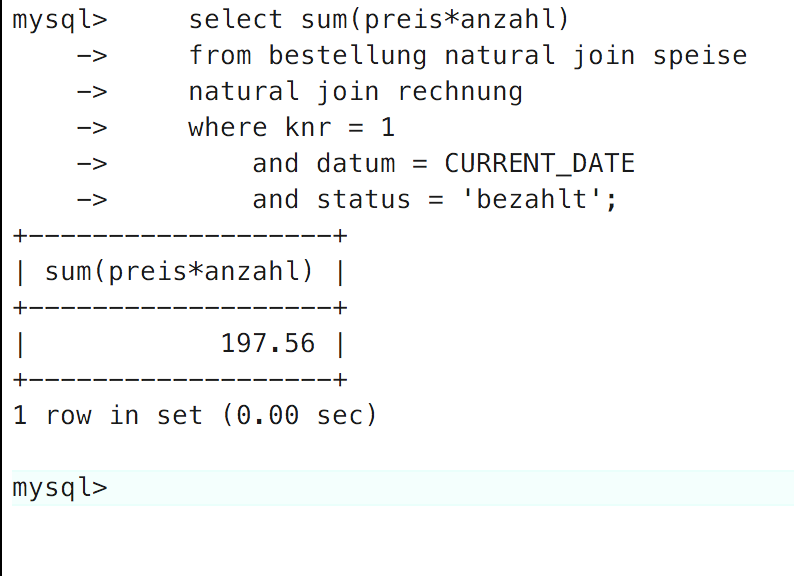
\includegraphics[width=1\linewidth]{images/s05.png}
\end{minipage}%
\begin{minipage}{.5\textwidth}
	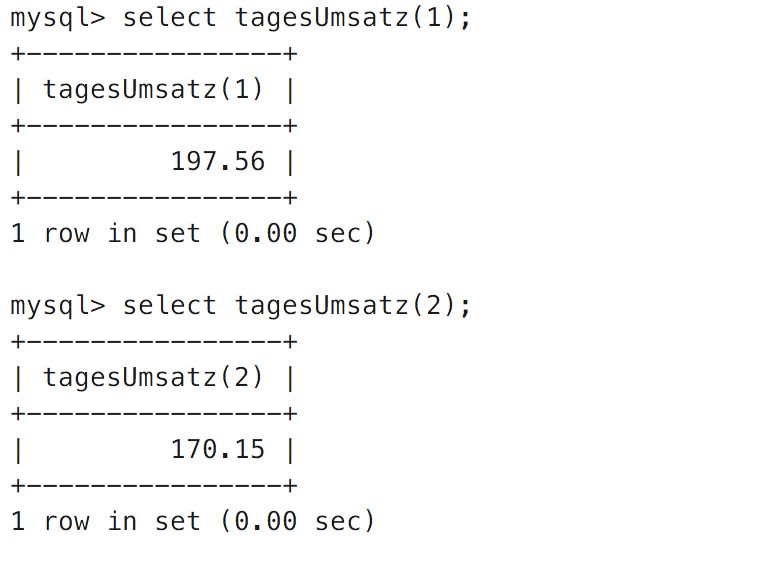
\includegraphics[width=1\linewidth]{images/s06.png}
\end{minipage}

\clearpage

\subsection{AU04 - Mehrwehrtssteuer}
\subsubsection{Umsetzung - \textit{mwst()}}
\vspace{0.3cm}
\begin{minipage}{.5\textwidth}
	\begin{lstlisting}[style=sql1, caption={mwst() - MySQL}]
DROP FUNCTION IF EXISTS bruttopreis;
CREATE FUNCTION bruttoPreis(preis DECIMAL(6,2))
	RETURNS DECIMAL(6,2) DETERMINISTIC
	RETURN (SELECT preis * 1.2);

DROP FUNCTION IF EXISTS mwst;
CREATE FUNCTION mwst(preis DECIMAL(6,2))
	RETURNS DECIMAL(6,2) DETERMINISTIC
	RETURN ( SELECT round(bruttoPreis(preis) - preis,2));

-- 			Aufruf
SELECT bezeichnung, preis as "Netto", bruttoPreis(speise.preis) as "Brutto", MwSt(speise.preis) as "MwSt"
FROM   speise;
	\end{lstlisting}
\end{minipage}%
\begin{minipage}{.5\textwidth}
	\begin{lstlisting}[style=sql, caption={mwst() - PSQL}]
CREATE OR REPLACE FUNCTION bruttoPreis(speise) RETURNS DECIMAL(6,2) AS $$
	SELECT round($1.preis * 1.2,2);
$$ LANGUAGE SQL;

--    MwST
CREATE OR REPLACE FUNCTION MwSt(speise) RETURNS DECIMAL(6,2) as $$
	SELECT round(bruttoPreis($1) - $1.preis,2)
	FROM   speise;
$$ LANGUAGE SQL;

SELECT bezeichnung, preis as "Netto", bruttoPreis(speise) as "Brutto", MwSt(speise) as "MwSt"
FROM   speise;
	\end{lstlisting}
\end{minipage}

\subsubsection{Bemerkungen}
Ähnlich wie bei psql wurden meherere Funktionen erstellt um ans Ziel zu kommen.
Letztendlich sieht der Aufruf sehr ähnlich aus und die Schwierigkeit der Funktionen ist sehr ähnlich.

\subsubsection{Screenshots}
	\begin{figure}[!h]
		\begin{center}
			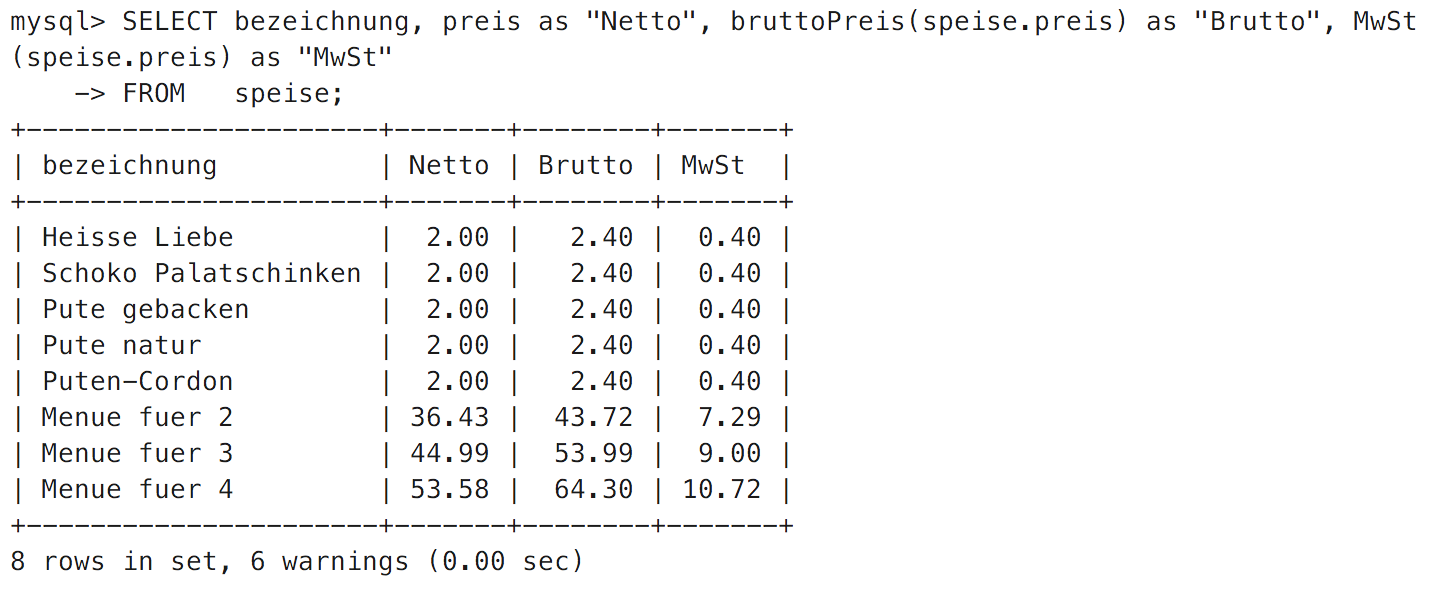
\includegraphics[width=0.65\linewidth]{images/s07.png}
		\end{center}
	\end{figure}

\clearpage

\subsection{AU05 - Noch nie bestellt}
\subsubsection{Umsetzung - \textit{mwst()}}
\vspace{0.3cm}
\begin{minipage}{.5\textwidth}
	\begin{lstlisting}[style=sql1, caption={nochNieBestellt() - MySQL}]
--	Noch nie Bestellte Speisen
--	sollen angezeigt werden.
DROP PROCEDURE IF EXISTS niebestellt;
DELIMITER $$
	CREATE DEFINER=CURRENT_USER PROCEDURE niebestellt()
	BEGIN
		SELECT bezeichnung AS "Bezeichnung", preis AS "Nettopreis"
		FROM speise
		WHERE speise.snr NOT IN (
			SELECT snr
			FROM bestellung
		);
	END $$
delimiter ;
	\end{lstlisting}
\end{minipage}%
\begin{minipage}{.5\textwidth}
	\begin{lstlisting}[style=sql, caption={nochNieBestellt() - PSQL}]
CREATE TABLE temp (
	"Bezeichnung" VARCHAR(255),
	"Nettopreis" DECIMAL(6,2)
);

CREATE OR REPLACE FUNCTION nieBestellt() 
	RETURNS SETOF temp AS $$
		SELECT bezeichnung AS "Bezeichnung", preis AS "Nettopreis"
		FROM speise
		WHERE speise.snr NOT IN (
			SELECT snr
			FROM bestellung
		);
	$$
LANGUAGE SQL;
	\end{lstlisting}
\end{minipage}

\subsubsection{Bemerkungen}
Hier wurde eine Prozedur gewählt da man ein set zurückgeben kann bzw. simulieren kann.
In psql wird hierbei eine temporäre Tabelle benötigt um das gleiche Ergebnis zu erreichen.

\subsubsection{Screenshots}
\begin{minipage}{.5\textwidth}
	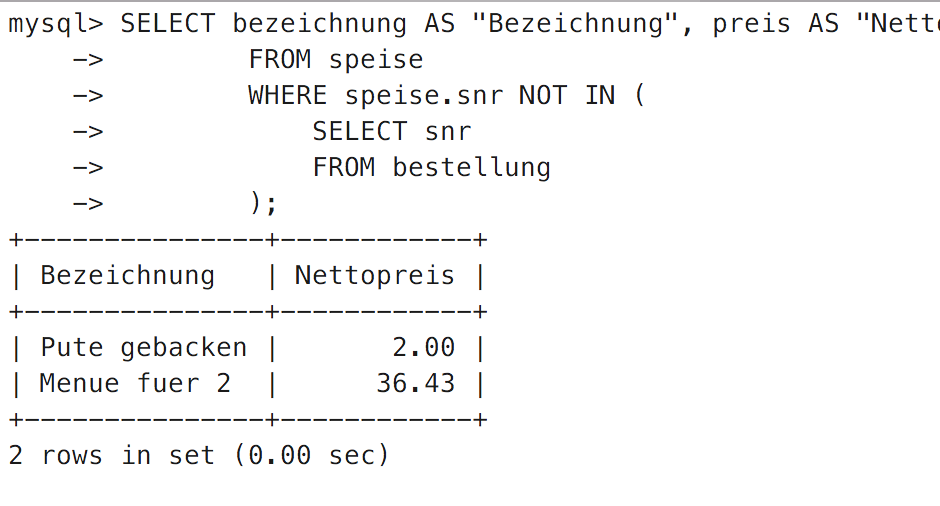
\includegraphics[width=1\linewidth]{images/s08.png}
\end{minipage}%
\begin{minipage}{.5\textwidth}
		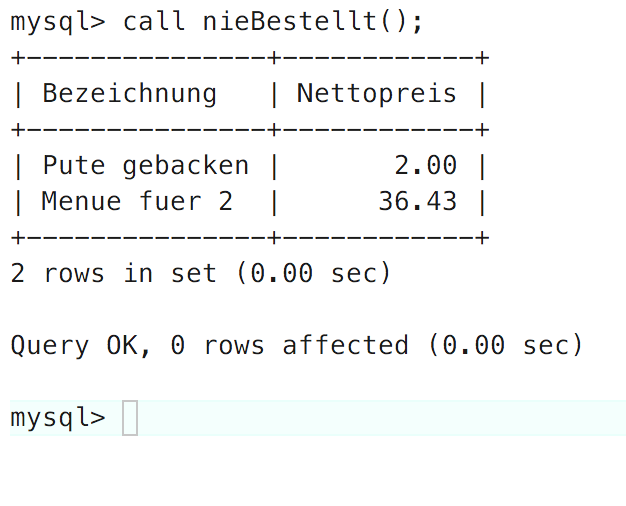
\includegraphics[width=0.7\linewidth]{images/s09.png}
\end{minipage}

\clearpage

\subsection{AU06 - Kellnerdaten}
\subsubsection{Umsetzung - \textit{kellnerdaten()}}
\vspace{0.3cm}
\begin{minipage}{.5\textwidth}
	\begin{lstlisting}[style=sql1, caption={kellnerdaten() - MySQL}]
drop function if exists anz_rechnungen;
create function anz_rechnungen(kellner INT)
	returns INT deterministic return
	(
		select count(*)
		from kellner natural join rechnung
		where kellner.knr = kellner
	);

drop function if exists spaeteste_rechnung;
create function spaeteste_rechnung(kellner INT)
	returns TEXT deterministic return
	(
		select status
		from rechnung
		where rechnung.knr = kellner
		order by rechnung.datum DESC
		limit 1
	);	
	
--	Aufruf
select name, anz_rechnungen(knr) as "Anzahl der Rechungen", spaeteste_rechnung(knr) as "Spaeteste Rechnung"
from kellner;
\end{lstlisting}
\end{minipage}%
\begin{minipage}{.5\textwidth}
	\begin{lstlisting}[style=sql, caption={kellnerdaten() - PSQL}]
--	Anzahl der Rechnungen
-- der Kellner
CREATE OR REPLACE FUNCTION anzRechnungen(INTEGER)
	RETURNS bigint AS $$
		select count(*)
		from kellner natural join rechnung
		where kellner.knr = $1;
	$$ Language sql;

-- Spaeteste Rechnung
-- des Kellners welcher mittels
-- paramter ausgewaehlt wurde
CREATE OR REPLACE FUNCTION spaetesteRechnung(INTEGER)
	RETURNS character AS $$
		select status
		from rechnung
		where rechnung.knr = $1
		order by rechnung.datum DESC
		limit 1;
	$$ Language sql;

--	Aufruf der obigen Funktionen
select name, anzRechnungen(knr) as "Anzahl der Rechungen", spaetesteRechnung(knr) as "Spaeteste Rechnung"
from kellner;
	\end{lstlisting}
\end{minipage}

\subsubsection{Bemerkungen}
Funktionen sind wiederum sehr ähnlich aufgebaut.
Es musste lediglich die Syntax der jeweiligen Funktion angepasst werden, wobei die parametisierung geändert werden musste, jedoch die grundsätzliche select anweisung unverändert gelassen worden konnte. 

\subsubsection{Screenshots}
\vspace{0.2cm}
	\begin{figure}[!h]
		\begin{center}
			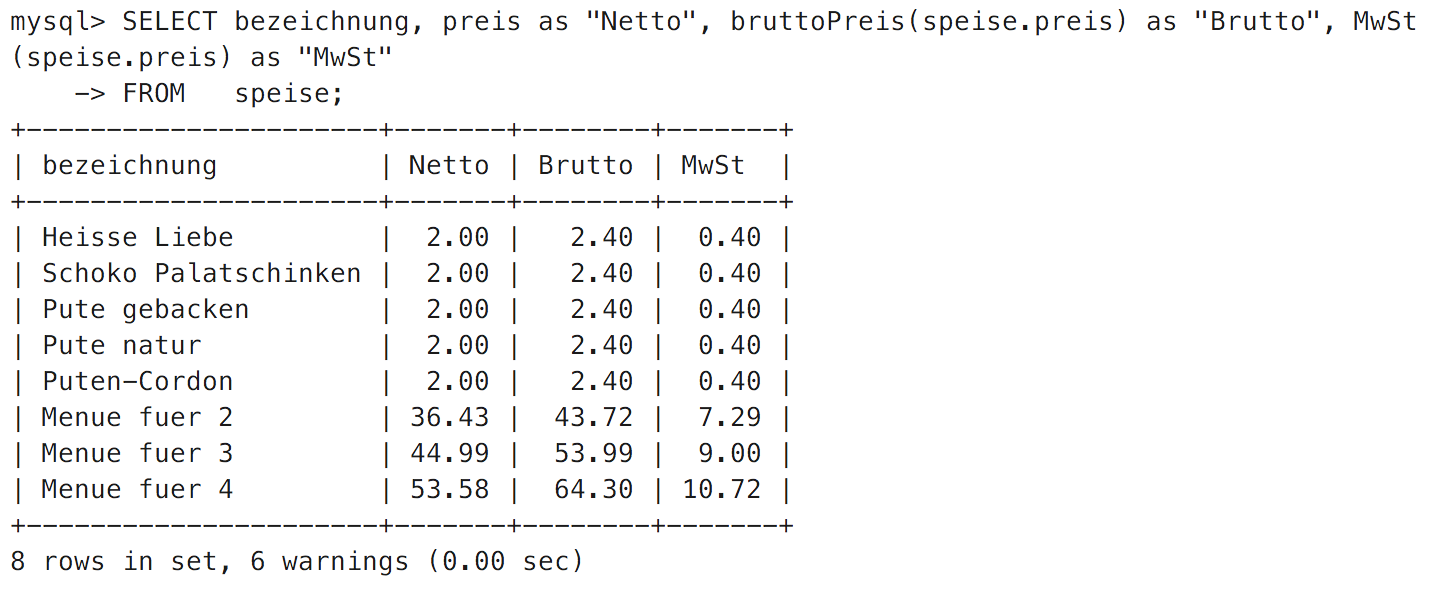
\includegraphics[width=0.65\linewidth]{images/s07.png}
		\end{center}
	\end{figure}

\clearpage

\subsection{AU07 - Tagesumsatz aller Kellner}
\subsubsection{Umsetzung - \textit{tagesumsatz\_pro\_kellner()}}
\vspace{0.3cm}
\begin{minipage}{.5\textwidth}
	\begin{lstlisting}[style=sql1, caption={tagesumsatzK() - MySQL}]
drop procedure if exists tagesumsatz_pro_kellner;
	delimiter $$
		create procedure tagesumsatz_pro_kellner()
		begin
			select name as "kname", sum(preis*anzahl)
			from bestellung 
				natural join speise 
				natural join rechnung
				natural join kellner
			where rechnung.status = 'bezahlt'
			group by name;
		end $$
	delimiter ;

-- 			Aufruf
call tagesumsatz-pro_kellner();
	\end{lstlisting}
\end{minipage}%
\begin{minipage}{.5\textwidth}
	\begin{lstlisting}[style=sql, caption={tagesumsatzK() - PSQL}]
create table temp (
kname VARCHAR(255),
kumsatz DECIMAL(6,2)
);

--          Funktion
--          @patam NONE
--          @return SETOF temp
create or replace function tagesumsatz()
returns setof temp as $$
select name as "kname", sum(preis*anzahl)
from bestellung natural join speise 
natural join rechnung
natural join kellner
where rechnung.status = 'bezahlt'
group by name;
$$ language sql;

select tagesumsatz();
	\end{lstlisting}
\end{minipage}

\subsubsection{Bemerkungen}
Es ist nicht möglich diese Aufgabe mithilfe von Functions zu lösen. Deshalb wurde auf Prozeduren zurückgegriffen.
Hierbei wurde letztendlich eine select anweisung aufgerufen und zurückgegeben, da eine Funktion in mysql nicht die Möglichkeit bietet ein set zurückzugeben.

In Psql wurde aufgrund dessen eine zusätzliche temporäre Tabelle entworfen um für den Zeitraum des Aufrufs die Datenaufteilung zu representieren damit sinnvolle Werte zurückgeliefert werden können.

\clearpage

\subsubsection{Screenshots}
\vspace{0.2cm}
\begin{minipage}{.5\textwidth}
	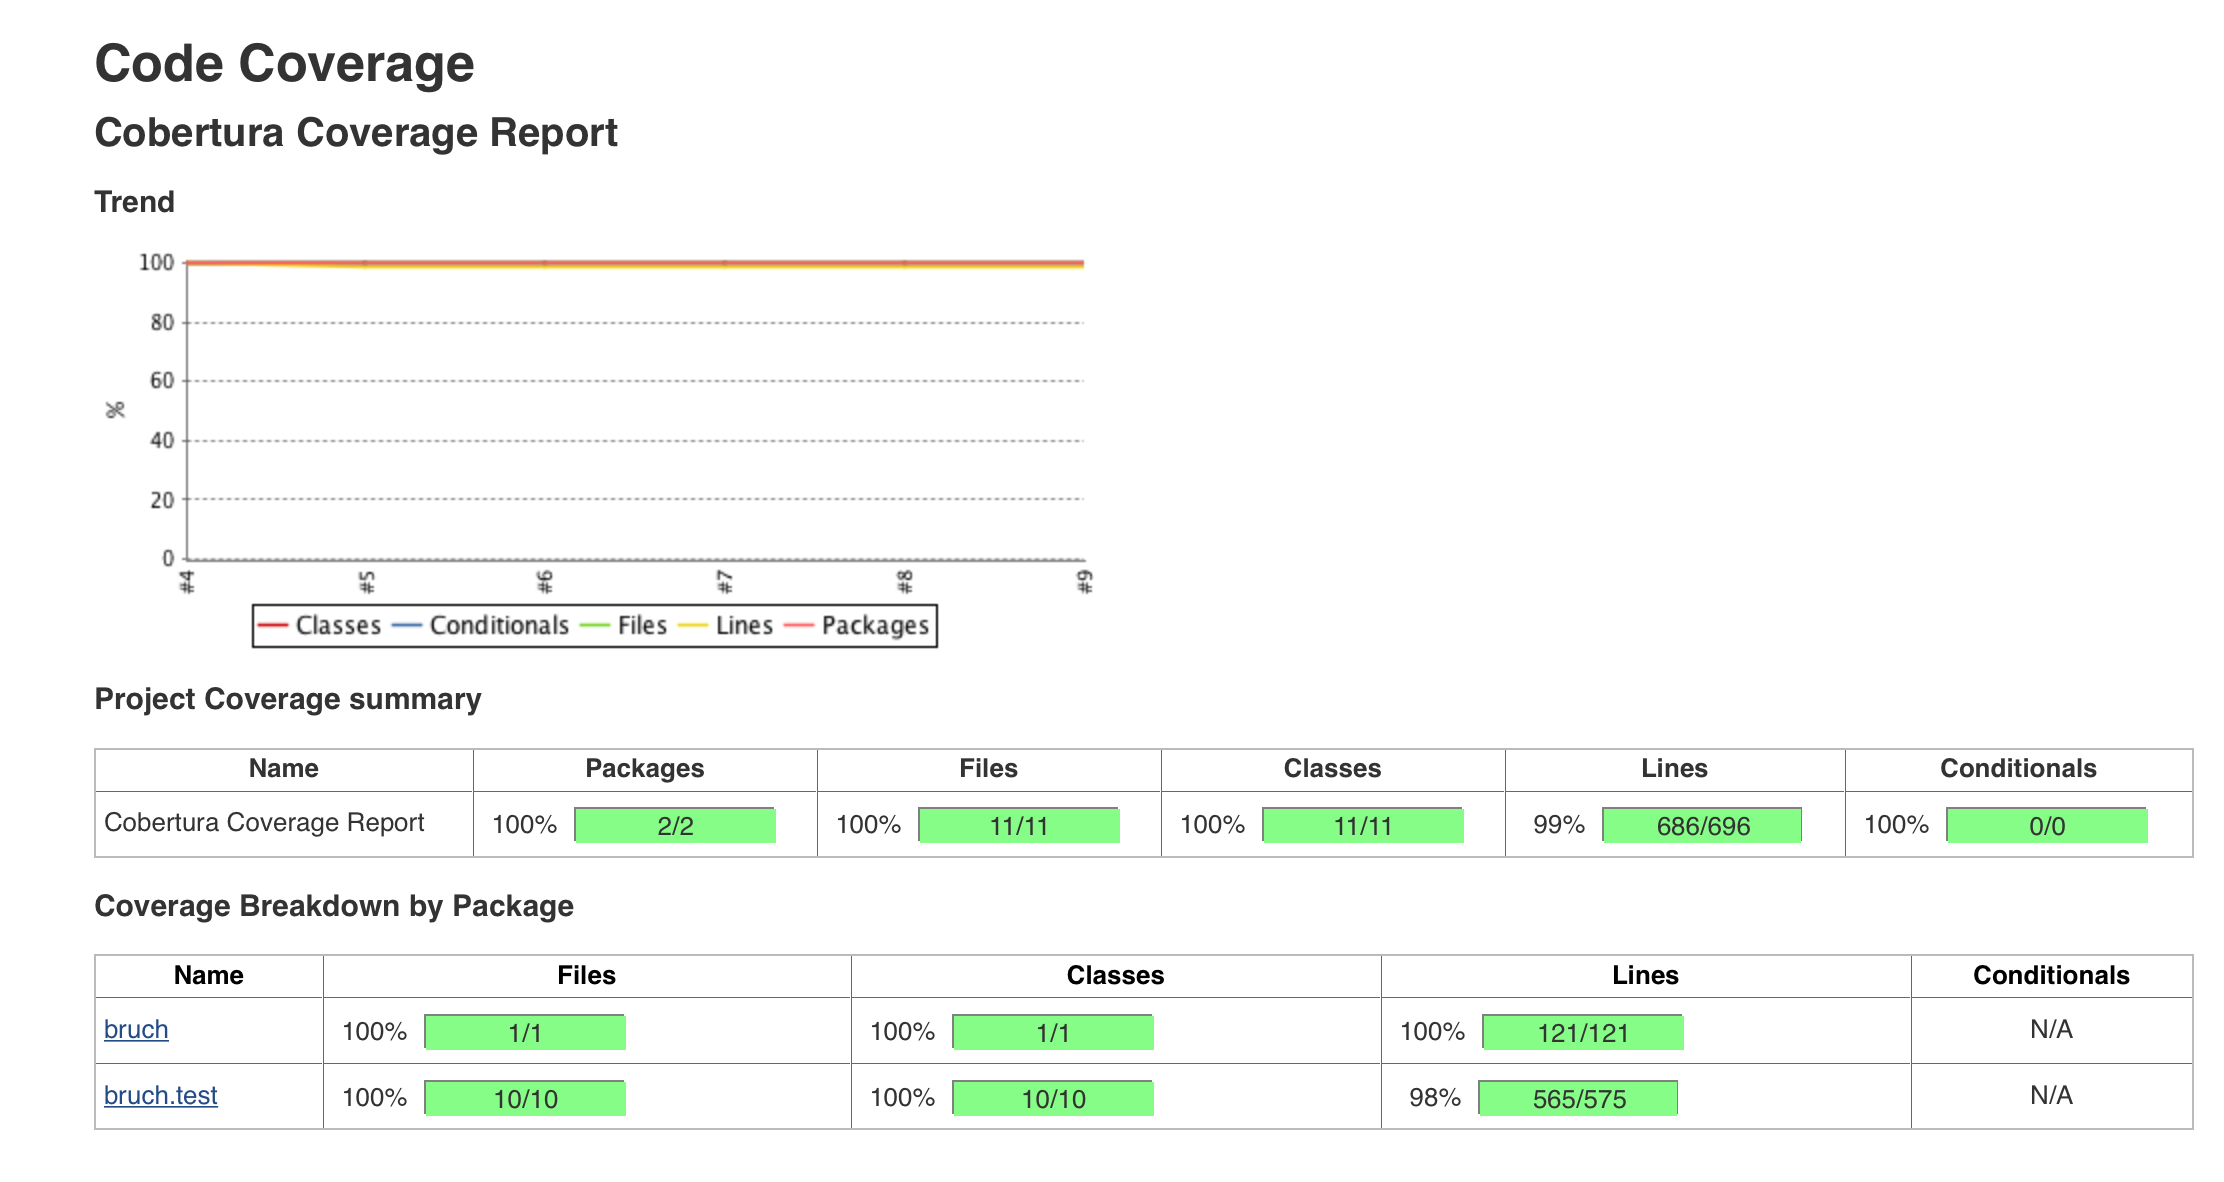
\includegraphics[width=1\linewidth]{images/s11.png}
\end{minipage}%
\begin{minipage}{.5\textwidth}
	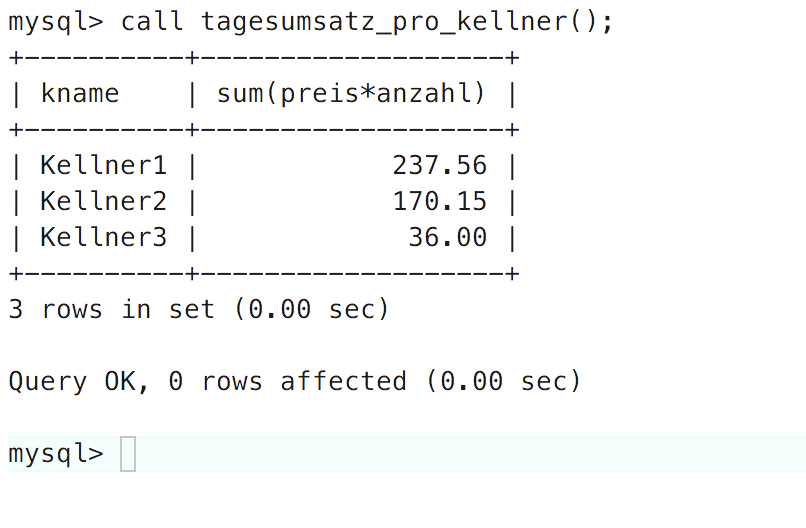
\includegraphics[width=1\linewidth]{images/s12.png}
\end{minipage}

\clearpage


